\documentclass[12pt]{article}

\usepackage[compact,small]{titlesec}
\usepackage[hmargin={0.6in,0.6in}, vmargin={0.5in, 0.01in}]{geometry}
\usepackage{graphicx, wrapfig, hyperref, url, denselists}
\usepackage{url, xcolor}
\newcommand{\email}[1]{\href{mailto:#1}{\normalfont\texttt{#1}}}


\usepackage{color}
\newcommand{\blue}[1]{{\textcolor{blue}{#1}}}
\newcommand{\red}[1]{{\textcolor{red}{#1}}}

\usepackage{enumitem}
\setitemize{noitemsep,topsep=0pt,parsep=0pt,partopsep=0pt}

\usepackage{graphicx}
\usepackage{transparent}
\usepackage{eso-pic}

\AddToShipoutPicture*{
    \put(0,0){
        \parbox[b][\paperheight]{\paperwidth}{%
            \vfill
            \centering
            {\transparent{0.15}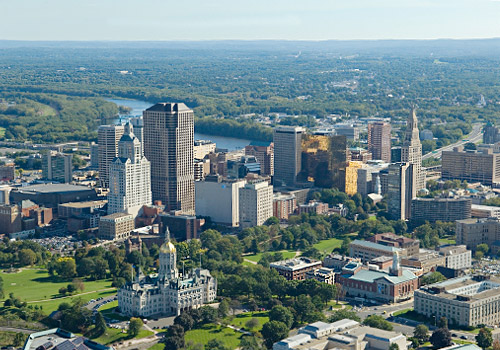
\includegraphics[height=\paperheight]{hartford}}%
            \vfill
        }
    }
}
\begin{document}

\pagestyle{empty}

\definecolor{dukeblue}{rgb}{0.0, 0.0, 0.61}

\noindent\fcolorbox{blue}{dukeblue}{%
\begin{minipage}[m]{1.8in}

\includegraphics[width=\linewidth]{NESS19}
\end{minipage}}%
\begin{minipage}[m]{5.5in}
\begin{center}
{\bf\Large  The 33rd New England Statistics Symposium\\[8pt]
 Statistical Data Science in Action}\\[8pt]
{\bf\large \url{https://symposium.nestat.org/}}\\[6pt]
{\bf\large Department of Statistics, University of Connecticut}\\[4pt]
{\bf May 15--17, 2019, Hilton Hartford, CT}
\end{center}
\end{minipage}

The Department of Statistics of the University of Connecticut is proud to host the first remodeled, 3-day NESS after the establishment of the New England Statistical Society, on May 15–17, 2019.

\paragraph{Four Short Courses}
Wednesday, May 15, 2019 (Course 1/2 are full-day while 3/4 are half-day)

% (\url{https://symposium.nestat.org/short-courses.html})

\noindent
1. %(Full-day)
Intermediate Machine Learning: Key Concepts and Techniques, by Dr. David Rosenberg (Bloomberg)

\noindent
2. %(Full-day)
Big Data Analytics and Deep Learning, by Dr. Ming Li (Amazon) and Dr. Hui Lin (Netlify)

\noindent
3. % (Half-day)
Practical Visualization for Data Scientists, by Dr. Xiaoyue Cheng (University of Nebraska at Omaha)

\noindent
4. %(Half-day)
Introduction to Multilevel Modeling, by Dr. Min Zhu (SAS)

\paragraph{Plenary Presentations} (\url{https://symposium.nestat.org/plenary-speakers.html})

\noindent\textsf{Opening Keynote} Thursday, May 16, 2019

Dr. Sam Kou, Harvard University: Big Data, Google and Disease Detection: A Statistical Adventure

Dr. David Rosenberg / Dr. Amanda Stent, Bloomberg: Machine Learning for Structured and Unstructured Data in Finance

\noindent\textsf{Banquet Talk} Thursday, May 16, 2019

Dr. Anthony D'Amico,   Dana-Farber Cancer Institute and Brigham \& Women's Hospital: Improving Patient Outcomes in Prostate Cancer by Partnering Statistics and Medicine

\noindent\textsf{Chernoff Lecture} Friday, May 17, 2019

The inaugural Chernoff Awardee whose identity remains a secret until the closing Award Ceremony.

\paragraph{Invited Sessions}
A total of 63 sessions cover a wide spectrum of areas of Statistical Data Science in Action. % with speakers from academia, industry, and government agencies. % Special panel discussions on career development and non-technical skills for statisticians and data scientists are of special interest to the next generation work force.
The schedule is online at \url{https://symposium.nestat.org/program.html}

\paragraph{Contributed Poster Session} Thursday, May 16, 2019.
Contribution is welcome from everyone.
Presenting students automatically enter the student poster award competition.

\paragraph{Student Competitions} Students are encouraged to participate in three events.

\textsf{Travelers Stat-a-thon} (\url{http://statathon.stat.uconn.edu/})
A statistical data science invention marathon sponsored by Travelers. Two data challenges have been released: Connecticut Housing; and Customer Retention. Students form teams to compete. The deadline of submission is April 26, 2019.

\textsf{IBM Student Paper Competition} Submission deadline is April 1, 2019.

\textsf{Liberty Mutual Student Poster Competition} Submission deadline is April 26, 2019.


\paragraph{Registration}
All participants in the conference must register. The registration fee
covers conference materials, breakfasts, lunches and tea
breaks. Members of the New England Statistical Society
(\url{https://nestat.org}) receive discounts in pricing. To register,
please complete the on-line registration form at
\url{https://symposium.nestat.org/registration.php}
by Monday, May 6, 2019.


\paragraph{Venue}
Hilton Hartford will offer discount rate to the conference
participants until April 18th or until the group block is sold out. To
book, please visit
\url{https://symposium.nestat.org/venue.html}.

\paragraph{Welcoming Reception}  5:00-6:30 pm, Wednesday, May 14.
Sponsored by Munich Re Group -- The Hartford
Steam Boiler Inspection and Insurance Co, free and open to all registered participants:

\vfill

\begin{center}

\includegraphics[width=\textwidth]{hartford-banner}
\end{center}


\newpage

\begin{center}
  {\bf\LARGE Highlights of the 33rd NESS, 2019\\[1ex]
    Statistical Data Science in \blue{\Huge Action}}\\[1ex]
  Detailed schedules of 60+ sessions at \url{https://symposium-dev.nestat.org/program.html}
\end{center}

In addition to the plenary sessions (keynote, banquet, Chernoff, and
award), a subset of parallel sessions themed with ``Statistical Data
Science in Actions'' are put in different tracks.

\paragraph{Travelers Stat-a-thon Finalist Presentations}
Finalists of the 2019 Travelers Stat-a-thon data challenges will
present their work in front of a judge panel on Thursday, May 16, in
two sessions, one on Connecticut Housing and the other on Customer
Retention. Winners will be presented with their prizes in the closing
award session on Friday, May 17, 2019.

\paragraph{Education and Career Development}
% Non-technical sessions that are accessible and beneficial to all
% statisticians and data scientists.
\begin{itemize}
\item
  % NESS19-IS-04
  % (Naitee Ting):
  Career Opportunities in Statistics and Data
  Sciences
\item
  % NESS19-IS-41
  % (Kathy Ziff):
  Effective Communication of Technical
  Concepts to Non-Technical Audiences
\item
  % NESS19-IS-54
  % (D. Betsy McCoach):
  Teaching Data Science
\item
  % NESS19-IS-66
  % (Sammi Tang):
  Leadership Forum for Statistics/Data Science Professionals
\end{itemize}

\paragraph{Showcase of Statistical Data Science in Action}
% Technical sessions (and organizers) that showcase a variety of
% actions of statistical data science.
\begin{itemize}
\item
  % NESS19-IS-62
  % (Tor D. Tosteson):
  Biomedical Data Science: To Infinity and Beyond!

\item
  % NESS19-IS-18
  % (Guojun Gan):
  Data Science in Actuarial Science

\item
  % NESS19-IS-42
  % (Nathan Lally):
  Data Science and Statistics in Insurance

\item
  % NESS19-IS-63
  % (Stavroula A. Chrysanthopoulou):
  Predictive Modeling in Data Science: Methods and Applications

\item
  % NESS19-IS-12
  % (Balgobin Nandram):
  Some Applications of Statistics in Data Science

\item
  % NESS19-IS-45
  % (Balaji Raman):
  Some Applications of Data Science in Industry

\item
  % NESS19-IS-55
  % (John Zhong):
  Application of Statistics and Data Sciences in Pharmaceutical
  Research and Development

\item
  % NESS19-IS-40
  % (Randy Paffenroth):
  Manifolds and Anomalies for Data Science

\item
  % NESS19-IS-57
  % (Kun Chen):
  The Role and Advances of Principled Statistical Inference in the Era
  of Data Science

\item
  % NESS19-IS-50
  % (Gregory J. Matthews):
  Sports Analytics % and Data Science

\item
  % NESS19-IS-23
  % (Jiwei Zhao):
  Novel Methodology and Application of Machine Learning Techniques in
  Data Science

\item
  % NESS19-IS-38
  % (Yasuo Amemiya):
  Data Science in Action at IBM Chief Analytics Office

\item
  % NESS19-IS-46
  % (Daoji Li):
  Novel Statistical Methods for Data Science: Discrete Data, Time
  Series and Data Integration

\item
  % NESS19-IS-53
  % (Tian Zheng):
  Robust Statistics for Data Science

\item
  % NESS19-IS-58
  % (Dakota Cintron):
  Data Science: Computational Social Science?

\item
  Using Statistics for Health Delivery System Reform in Massachusetts
\item
  Healthcare Data Analysis for Electronic Health Records
\item
  Statistical Methodology for Healthcare Data Analysis
\item
  Novel Statistical Methods for the Analysis of Genomic Data
\item
  Air Pollution and Public Health %: New Spatial and Spatio-Temporal
  % Statistical Approaches for Exposure Assessment and Causal Inference
\item
  Statistical Tools for Addressing the Opioid Epidemic
\item
  Modern Statistical Methods for Health Outcome Data
\item
  Critical Questions in Drug development
\item
  Statistical and Machine Learning Methods for Large-Scale Biomedical
  Data Analysis
\end{itemize}



\paragraph{Probability, Statistics, and Geometry: A Special Session
  Honoring Professor Rick Vitale}
This session is to honor Professor Rick Vitale for
his academic achievements and to celebrate his 75th birthday.
Chaired by \textsf{David Pollard} (Yale University),
it starts at 1:00 pm on Friday, May 17:
\begin{itemize}
\item
\textsf{Andrew Barron} (Yale University): Gaussian Complexity, Metric
Entropy, and Risk of Deep Nets
\item
\textsf{David Donoho}  (Stanford University): The Statistical
Significance of Perfect Linear Separation
\item
\textsf{Subhashis Ghoshal} (North Carolina State University): Coverage
of Credible Intervals for Monotone Regression
\end{itemize}

\end{document}

